\documentclass{article}
\usepackage[utf8]{inputenc}
\usepackage{enumerate}
\usepackage{amsmath}
\usepackage{amssymb}
\usepackage{amsfonts}
\usepackage{amstext}
\usepackage{amsthm}
\usepackage{mathtools}
\usepackage{tikz}
\usepackage{tikz-3dplot}
\usetikzlibrary{angles, quotes}
\usepackage{amssymb}
\usepackage{amsmath}
\usepackage{cancel}
\DeclarePairedDelimiter{\ceil}{\lceil}{\rceil}
\title{Calculus III Review Sheet 1 Practice}
\author{Eddie Ozuna,Tyler Franklin}

\begin{document}
\maketitle

Recall that the dot product of two vectors $\vec{u}$ and $\vec{v}$ may be denoted by any of
the expressions " $\vec{u}\cdot \vec{v}$ ", " $<\vec{u}, \vec{v}>$ ", " $\vec{u}^T \vec{v}$ ", and is also referred to as “the inner product”.
\\
\\
The cross product of two vectors u and v will be denoted “ $\vec{u}\times\vec{v}$ ”.
Also, recall that the length of any vector $\vec{u}$ is denoted by $\mid\vec{u}\mid$.
\\
\\
Throughout this review, lets establish the following notation:\\
\\
\\
$\vec{u}=\left(\!\begin{array}{c}u_{1} \\ u_{2} \\  u_{3}\end{array} \!\right)$,
$\vec{v}=\left(\!\begin{array}{c}v_{1} \\ v_{2} \\  v_{3}\end{array} \!\right)$,
$\vec{w}=\left(\!\begin{array}{c}w_{1} \\ w_{2} \\  w_{3}\end{array} \!\right)$
\\
\\
\\
$e_{1}=\left(\!\begin{array}{c}1 \\ 0 \\  0\end{array} \!\right)$,
$e_{2}=\left(\!\begin{array}{c}0 \\ 1 \\  0\end{array} \!\right)$,
$e_{3}=\left(\!\begin{array}{c}0 \\ 0 \\  1\end{array} \!\right)$
\\
\\
\\
\begin{enumerate}[1.]
\item\textbf{Prove that for any two vectors u and v, the inner product of u and v is equal to $\mid\vec{u}\mid\mid\vec{v}\mid\cos(\theta)$ where $\theta$ is the angle between $\vec{u}$ and $\vec{v}$.\\\\Hint: Draw the picture and recall the Law of Cosines is just a degeneration of
the Pythagorean Theorem:}\\
\\
Derivation: Law of Cosine\\
	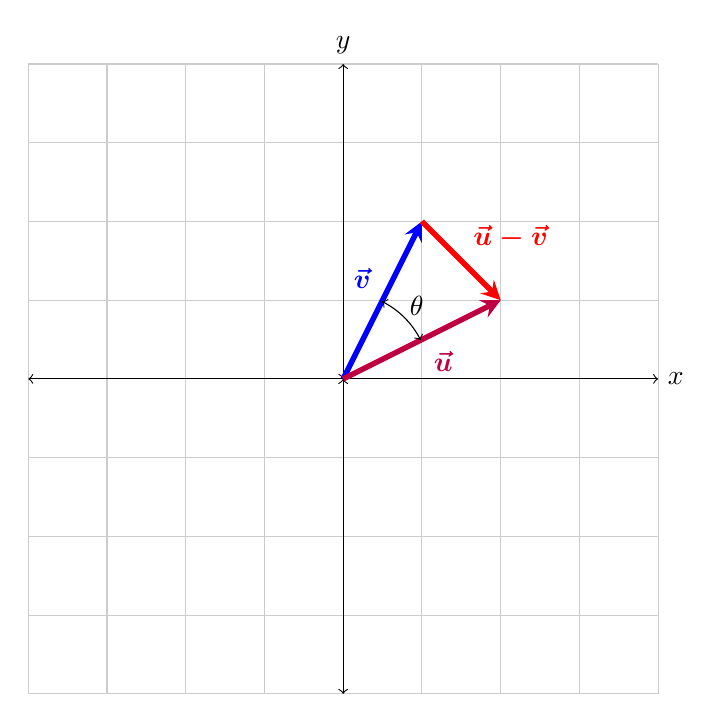
\begin{tikzpicture}
  \draw[thin,gray!40] (-4,-4) coordinate (o) grid (4,4);
  \draw[<->] (0,0)--(0,0) coordinate (o) node[right]{};
  \draw[<->] (-4,0)--(4,0)  node[right]{$x$};
  \draw[<->] (0,-4)--(0,4)  node[above]{$y$};
  \draw[line width=2pt,blue,-stealth](0,0)--(1,2) coordinate (x) node[midway,auto]{$\boldsymbol{\vec{v}}$};
  \draw[line width=2pt,purple,-stealth](0,0)--(2,1) coordinate (y) node[midway,auto,swap]{$\boldsymbol{\vec{u}}$};
  \draw[line width=2pt,red,-stealth](1,2)--(2,1) node[midway,auto]{$\boldsymbol{\vec{u}-\vec{v}}$};
 \pic [draw, <->,
      angle radius=11mm, angle eccentricity=1.2,
      "$\theta$"] {angle = y--o--x};
\end{tikzpicture}\\
$\mid\vec{u}-\vec{v}\mid^{2} = \mid\vec{u}\mid^{2} + \mid\vec{v}\mid^{2}-\hspace{.1cm}2\mid\vec{u}\mid\cdot\mid\vec{v}\mid\cos(\theta)$\\
\\
$\cancel{\mid\vec{u}\mid^{2}}-\hspace{.1cm}2\vec{v}\cdot\vec{u}\hspace{.1cm}+\cancel{\mid\vec{v}\mid^{2}}=\cancel{\mid\vec{u}\mid^{2}} + \cancel{\mid\vec{v}\mid^{2}}-2\mid\vec{u}\mid\cdot\mid\vec{v}\mid\cos(\theta)$\\
\\
$\cancel{-2}\vec{v}\cdot\vec{u} = \cancel{-2}\mid\vec{u}\mid\cdot\mid\vec{v}\mid\cos(\theta)$\\
\\
$\vec{v}\cdot\vec{u} = \mid\vec{u}\mid\cdot\mid\vec{v}\mid\cos(\theta)$\\
\end{enumerate}
\begin{enumerate}[2.]
\item\textbf{Are the vectors $\vec{u}=\left(\!\begin{array}{c}1 \\ 2 \\  3\end{array} \!\right)$ , $\vec{v}=\left(\!\begin{array}{c}-2 \\ 1 \\  0\end{array} \!\right)$ orthogonal? Why or why not?}\\
\\
Vectors are orthogonal(perpendicular) if and only if the result of the dot product is zero.\\
\\
($\vec{u}\cdot\vec{v})=(1\cdot-2)+(2\cdot1)+(3\cdot0)=0$
\\
\\
Yes they are orthogonal 
\end{enumerate}
\begin{enumerate}[3.]
\item\textbf{Prove that the cross product of two vectors $\vec{u}$ and $\vec{v}$ is actually orthogonal to each of $\vec{u}$ and $\vec{v}$ simultaneously, i.e. $\vec{u}\times\vec{v}$ is orthogonal to $\vec{u}$ and $\vec{u}\times\vec{v}$ is
orthogonal to $\vec{v}$ }
\\
\\
Step 1. Take the cross product of $\vec{u}$ and $\vec{v}$\\
\\
$\vec{u}\times\vec{v}=\begin{vmatrix}
\hat{i}&\hat{j}&\hat{k}\\
u_{1}&u_{2}&u_{3}\\
v_{1}&v_{2}&v_{3}\\
\end{vmatrix}=\hat{i}
\begin{vmatrix}
u_{2}&u_{3}\\
v_{2}&v_{3}\\
\end{vmatrix}-\hat{j}\begin{vmatrix}
u_{1}&u_{3}\\
v_{1}&v_{3}\\
\end{vmatrix}+\hat{k}\begin{vmatrix}
u_{1}&u_{2}\\
v_{1}&v_{2}\\
\end{vmatrix}\\
=\hat{i}(u_{2}v_{3}-u_{3}v_{2})-\hat{j}(u_{1}v_{3}-u_{3}v_{1})+\hat{k}(u_{1}v_{2}-u_{2}v_{1})$\\
\\
Let define $\vec{w}$ to be equal to the result of the cross product of $\vec{u}$ and $\vec{v}$\\
\\
Step 2. From our previous knowledge we know that if the result of the dot product is zero the vectors are orthogonal(perpendicular). With that being said let perform the dot products of vector $\vec{u}$ with $\vec{w}$ and $\vec{v}$ with $\vec{w}$.\\
\\
$\vec{w} = <(u_{2}v_{3}-u_{3}v_{2}),-(u_{1}v_{3}-u_{3}v_{1}),(u_{1}v_{2}-u_{2}v_{1})>$\\
\\
$\vec{u}\cdot\vec{w}=u_{1}(u_{2}v_{3}-u_{3}v_{2})-u_{2}(u_{1}v_{3}-u_{3}v_{1})+u_{3}(u_{1}v_{2}-u_{2}v_{1})\\=u_{1}u_{2}v_{3}-u_{1}v_{2}u_{3}-u_{1}u_{2}v_{3}+v_{1}u_{2}u_{3}+u_{1}u_{3}v_{2}-v_{1}u_{2}u_{3}=0$\\
\\ 
$\vec{v}\cdot\vec{w}=v_{1}(u_{2}v_{3}-u_{3}v_{2})-v_{2}(u_{1}v_{3}-u_{3}v_{1})+v_{3}(u_{1}v_{2}-u_{2}v_{1})\\=v_{1}u_{2}v_{3}-v_{1}v_{2}u_{3}-u_{1}v_{2}v_{3}+v_{1}v_{2}u_{3}+u_{1}v_{2}v_{3}-v_{1}u_{2}v_{3}=0$\\
\\
Proven Both yield a result of zero which state they are orthogonal(perpendicular) simultaneously.
\end{enumerate}
\begin{enumerate}[4.]
\item\textbf{Find a vector that is orthogonal to each of the vectors $1\cdot e_{1}+1\cdot e_{2}+1\cdot e_{3}$ and $1\cdot e_{1}+1\cdot e_{2}+0\cdot e_{3}$. Prove that your vector is actually perpendicular to
each of $e_{1}$ and $e_{2}$ simultaneously}\\
\\
Step 1. Simplify $1\cdot e_{1}+1\cdot e_{2}+1\cdot e_{3}$ and $1\cdot e_{1}+1\cdot e_{2}+0\cdot e_{3}$.\\
\\
$1\cdot e_{1}+1\cdot e_{2}+1\cdot e_{3}=1\cdot<1,0,0>+1\cdot<0,1,0>+1\cdot<0,0,1>\\=<1\cdot1,1\cdot0,1\cdot0>+<1\cdot0,1\cdot1,1\cdot0>+<1\cdot0,1\cdot0,1\cdot1>\\=<1,0,0>+<0,1,0>+<0,0,1>\\=<1+0+0,0+1+0,0+0+1>=<1,1,1>$\\
\\
$1\cdot e_{1}+1\cdot e_{2}+0\cdot e_{3}=1\cdot<1,0,0>+1\cdot<0,1,0>+0\cdot<0,0,1>\\=<1\cdot1,1\cdot0,1\cdot0>+<1\cdot0,1\cdot1,1\cdot0>+<0\cdot0,0\cdot0,0\cdot1>\\=<1,0,0>+<0,1,0>+<0,0,0>\\=<1+0+0,0+1+0,0+0+0>=<1,1,0>$

Let $\vec{p}$ and $\vec{q}$ equal to the result we got.\\
\\
$\vec{p}=<1,1,1>$
\\
$\vec{q}=<1,1,0>$\\
\\
Step 2. Take the cross product of vector $\vec{p}$ with $\vec{q}$\\
\\
$\vec{p}\times\vec{q}=\begin{vmatrix}
\hat{i}&\hat{j}&\hat{k}\\
1&1&1\\
1&1&0\\
\end{vmatrix}=\hat{i}
\begin{vmatrix}
1&1\\
1&0\\
\end{vmatrix}-\hat{j}\begin{vmatrix}
1&1\\
1&0\\
\end{vmatrix}+\hat{k}\begin{vmatrix}
1&1\\
1&1\\
\end{vmatrix}\\=\hat{i}(1\cdot0-1\cdot1)-\hat{j}(1\cdot0-1\cdot1)+\hat{i}(1\cdot1-1\cdot1)=-1\hat{i}+1\hat{j}+0\hat{k}$\\
\\
Let $\vec{r}$ equal to the result we got.\\
\\
$\vec{r} = <-1,1,0>$\\
\\
Step 3. Take the dot product of $\vec{e_{1}}$ with $\vec{r}$  and $\vec{e_{2}}$ with $\vec{r}$ to see if they are orthogonal simultaneously\\
\\
$\vec{e_{1}}\cdot\vec{r}=(1\cdot-1)+(1\cdot1)+(1\cdot0)=0$
\\
\\
$\vec{e_{2}}\cdot\vec{r}=(1\cdot-1)+(1\cdot1)+(0\cdot0)=0$
\\
\\
Proven Both yield a result of zero which state they are orthogonal(perpendicular) simultaneously.
\end{enumerate}
\end{document}